\chapter{Interoperability}
Merkle proofs from \ref{merkle:inclusion} are used to prove to a light client that a transaction has happened. \\
\textbf{Now this can be used to prove to blockchain B that a transaction like a token transfer has taken place in a blockchain A.}

In this chapter let's see how interoperability between blockchains can be achieved using merkle proofs. 

\section{Interoperability with merkle proofs}
\subsection{Definition}
Interoperability has many different definitions. 
For example, \cite{wegner1996interoperability} defines it as the ability of two or
more software components to cooperate
despite differences in language, 
interface, and execution platform.

Now blockchain interoperability can be defined by the ability of different blockchain networks to communicate and exchange data with each other.


\subsection{Token transfer workflow}
\begin{figure}[H]
    \centering
    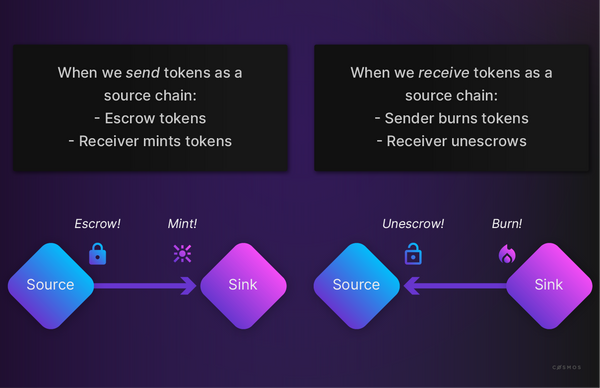
\includegraphics[width=0.5\linewidth]{interoperability/transfer_token.png}
    \caption{Token transfer (from cosmos)}
    \label{fig:token_transfer}
\end{figure}
\begin{enumerate}
    \item The user from source chain send his tokens to the receiver to an escrow contract deployed on the source chain. 
    \item Full nodes of chain A monitor these events usually
    \item they generate the merkle proof for the transaction of these escrowed tokens
    \item the blockchain B receives, somehow, the proof that the transaction happened along with the block header of this transaction
    \item blockchain B can then be sure that the transaction happened and mint the equivalent tokens to the receiver.
\end{enumerate}



\subsection{Expressivity}
The question is how well can you describe the source chain in order to trigger actions in the destination chain?
In bitcoin we just have a binary merkle root of the transactions. It means that you can only prove the inclusion of the transactions. 
How many bitcoins do you have? It's not a question you can answer with the merkle root in bitcoin because it only describes the transactions. 
In ethereum in contrast, as explained here \ref{merkle:ethereum} there are three trees saved. One for the transactions as in bitcoin, one for the state, and one for the receipts. 


\textbf{
These merkle trees allows Ethereum to answer more questions than just the inclusion of a transaction.
}

For example:
\begin{itemize}
\item Has this transaction been included in a particular block?
\item What is the current balance of my account?
\item Does this account exist?
\item Tell me all instances of an event of type X (eg. a crowdfunding contract reaching its goal) emitted by this address in the past 30 days
\item Pretend to run this transaction on this contract. What would the output be?
\end{itemize}

The first one can be answered by the transactions tree as in bitcoin, the second and the third by the state tree, the fourth by the receipt tree. The fifth is a bit more complicated but can be proven by the state tree also. 


Obviously Ethereum offers much more functionalities than bitcoin, and these trees offer the ability to describe Ethereum world more precisely. 

This is relevant for the interoperability challenges. You can now react in the destination chain to a lot more information from the source chain. 

\section{Examples}
So, now that we understand the merkle proofs, \textbf{how are they used in current interoperability solutions?}
\\We present a rapid overview of some interesting solutions, the goal here is to understand where the merkle proofs step in and how they help achieving interoperability in these protocols, leaving many details uncovered to keep it simple.

In \ref{background:security}, we highlight that the security of the light client relies on having the verified block headers. The following protocols use different techniques to prove that the block headers are valid. 

\subsection{LayerZero \cite{zarick2021layerzero}}
\begin{figure}[H]
    \centering
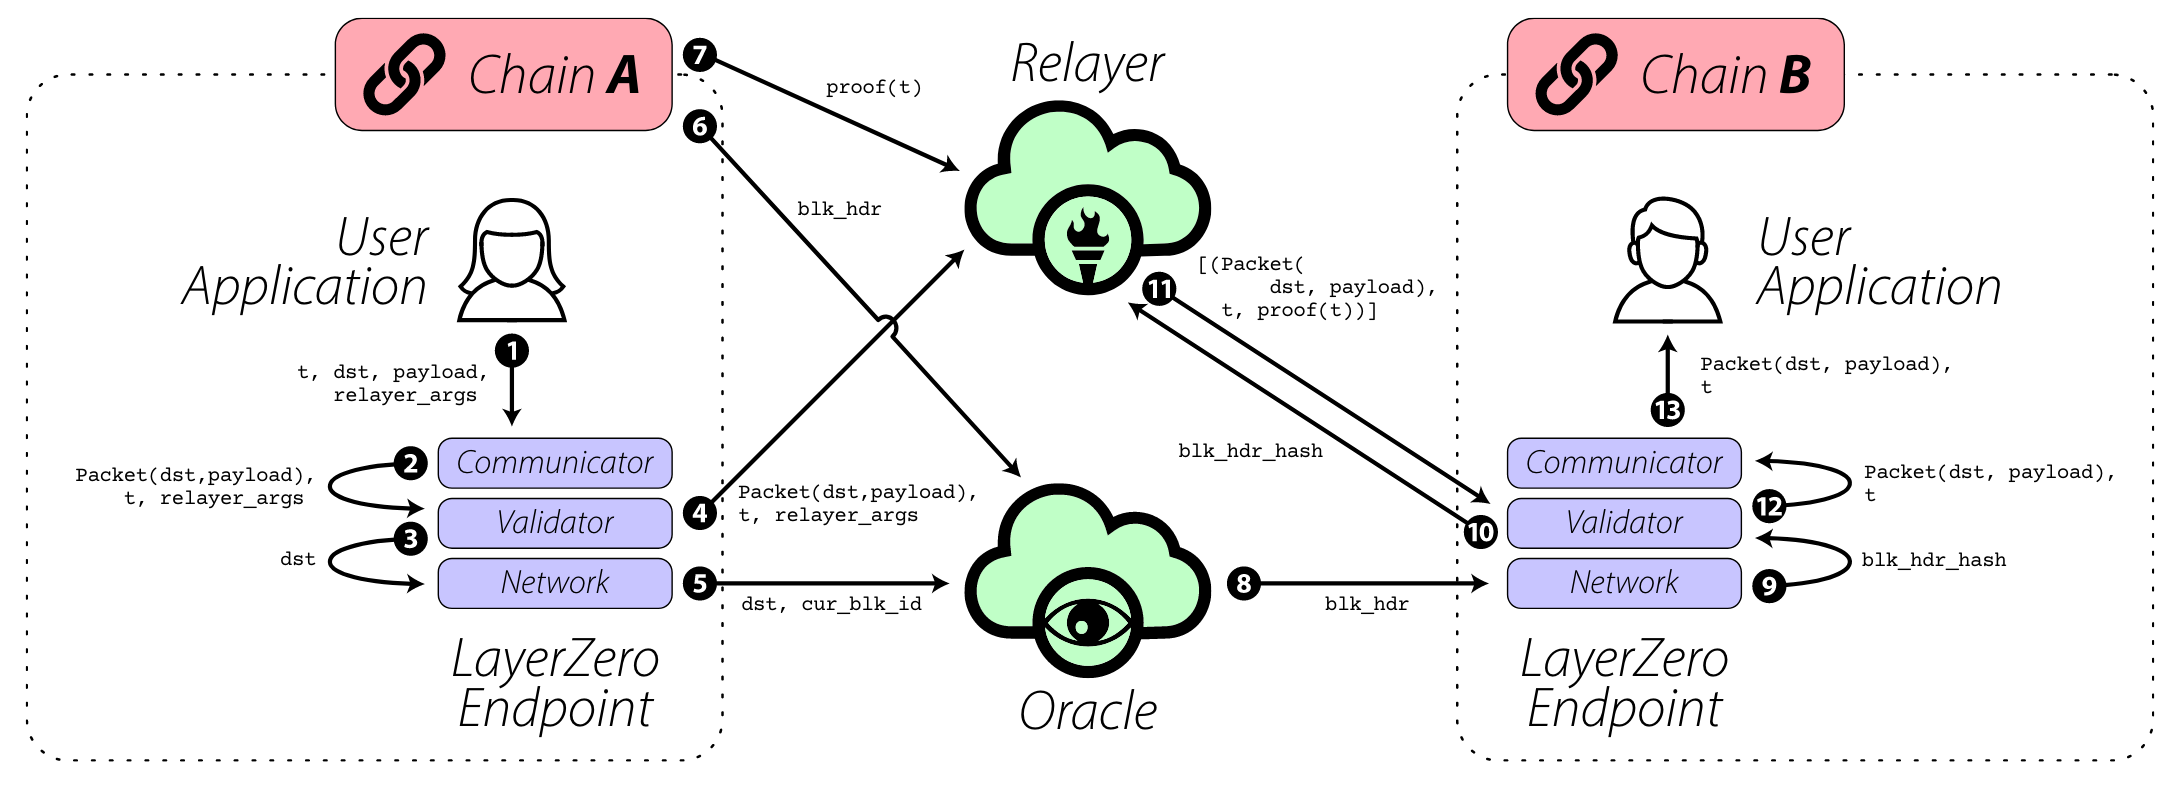
\includegraphics[width=1.\linewidth]{interoperability/layerZero.png}
    \caption{LayerZero}
    \label{fig:layer_zero}
\end{figure}

For each supported chain, LayerZero deploys an endpoint, consisting in 4 smart contracts. This endpoint includes a library handling the verification of the transaction proof.

So, from \ref{merkle:inclusion},  to verify that a transaction has taken place we need the merkle root, included in the block header and the the merkle proof. 
\\
LayerZero offers interoperability by transporting these two necessary pieces of data.
\begin{itemize}
    \item The block header containing the merkle root is carried by the oracle from blockchain A to blockchain B. 
    \item The merkle proof of blockchain A is carried by a relayer from blockchain A to blockchain B.
\end{itemize}

The oracle is a Chainlink oracle monitoring the source blockchain and the relayer can be handled by LayerZero or anyone interested into this. 
\\
Chain B can then attest that the transaction has happened by verifying the proof against the block header sent by the oracle.

\textbf{The security of LayerZero relies on the independence of the relayer and the oracle.}

If the oracle and the relayer collude, they can give a fake block header, and a proof working with that fake block. 


\subsection{ZKBridge \cite{xie2022zkbridge}}
\begin{figure}[H]
    \centering
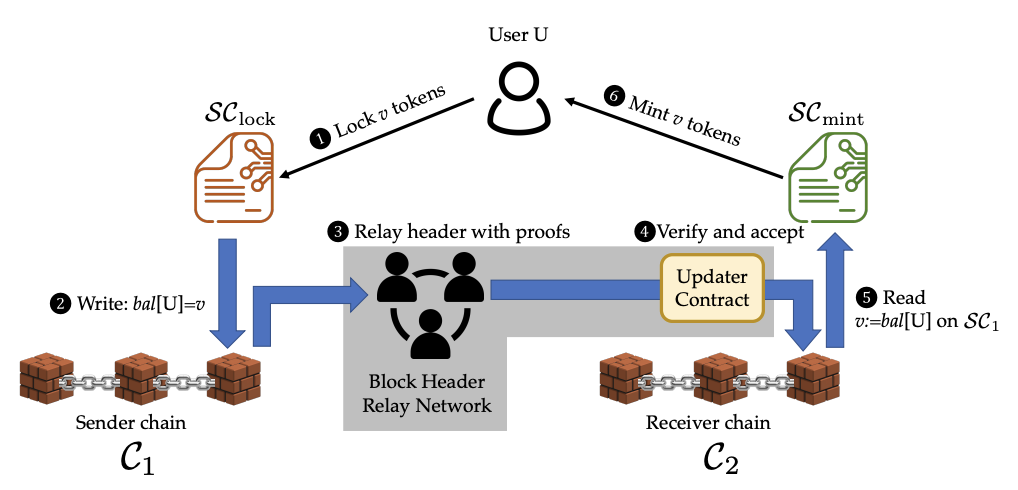
\includegraphics[width=0.8\linewidth]{interoperability/zkbridge.png}
    \caption{ZKbridge}
    \label{fig:zkbridge}
\end{figure}

Zero knowledge proofs are introduced here: \ref{zeroknowledge}.

So here, the gray part is ZKbridge.
\\The most important part is done here by the relayers. 
\begin{enumerate}
    \item The relayers contact the full nodes of blockchain C1 to get the last block header% $blkH_r$ following the $blkH_{r-1}$
    \item the relayers generate a zero knowledge proof that a light client of the sender chain C1 accepts that block header
    \item This proof is then sent to the ZKBridge updater contract of the receiving chain C2
    \item this updater contract verifies the ZK proof and adds it to its list of block headers if successfully verified.
    \item The application contract, anyone on C2 can call the public function GetHeader from the updater contract to get the header. 
\end{enumerate}

Zk bridge achieve interoperability by verifying the validity of the block header. The relayers do that in a indirect way : they prove by a zk proof that a light client of the source chain accepts this block header. 
\\
Let's understand what the acceptance of the light client means. 
In ethereum, it means that: 
\begin{itemize}
    \item the status of the block header is finalized. Finality means that you can be sure it'll not be reverted. 
    \item the sync committee, group of validators, have sufficient participants 
    \item the aggregated signature is correct, meaning that the aggregator in Ethereum received enough votes and signed it.
\end{itemize}
In \cite{ethereumlcvalidation}, you can directly check the code for validating the light client update, the acceptance of the block header.  
\begin{figure}[H]
    \centering
    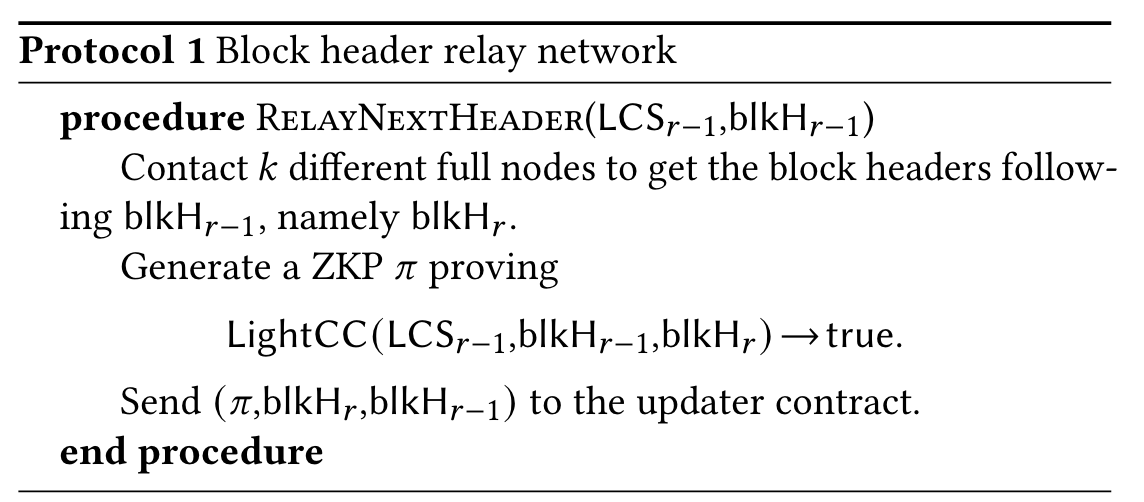
\includegraphics[width=0.6\linewidth]{interoperability/zkbridgeprotocol.png}
    \caption{Relayer protocol}
    \label{fig:zkbrigdeprotocol}
\end{figure}

\textbf{The security of the ZKbridge relies notably on the security of the light client of C1.} It's because the zero knowledge proof consists in proving that this light client accepts the block.

\subsection{Telepathy \cite{telepathy}}

\begin{figure}[H]
    \centering
    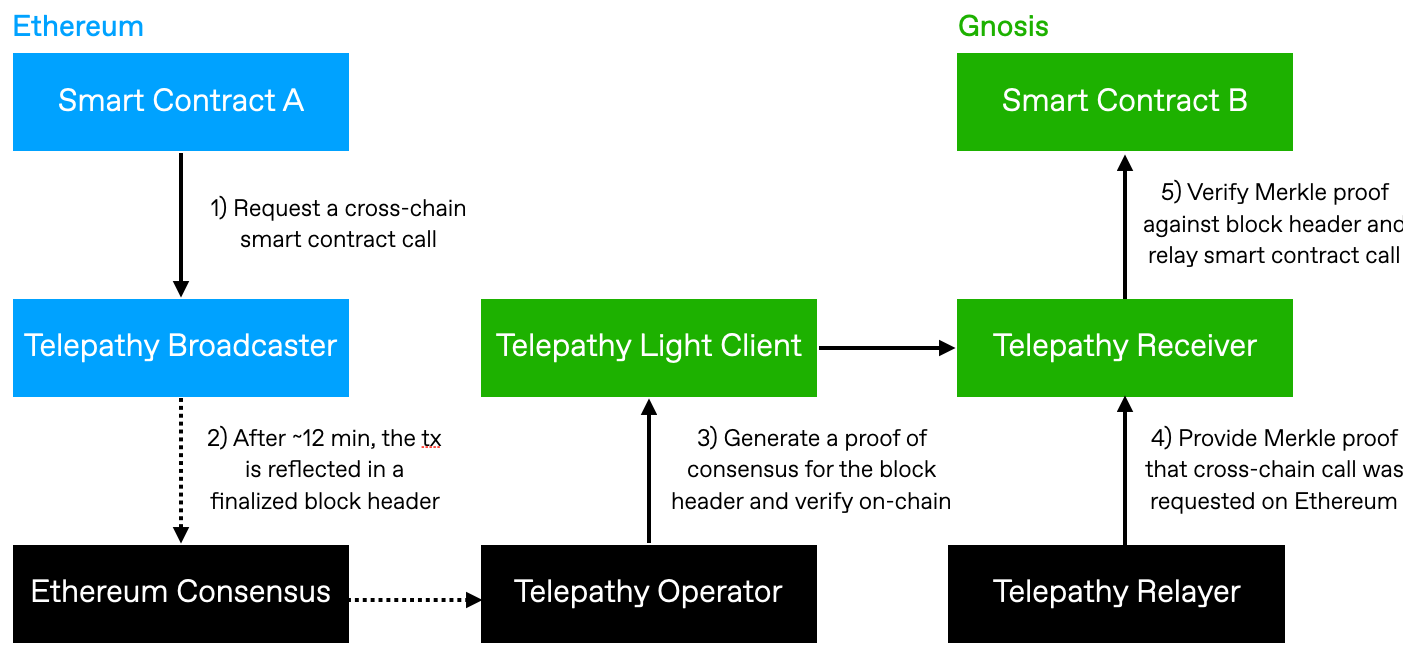
\includegraphics[width=0.8\linewidth]{interoperability/telepathy.png}
    \caption{Telepathy workflow}
    \label{fig:telepathy}
\end{figure}

Telepathy is based on proof of consensus. It means that to prove that a block header from blockchain A is valid, it will basically check that a large majority of the validators signed the block header. 
More precisely, the 2.0 Ethereum has a sync committee of 512 validators randomly chosen every 27 hours and is responsible for signing every block header during that period. If at least 2/3 of the validators sign a given block header, the block is considered finalized and the network state is valid. 

But verifying all these signatures one by one is computationally expensive. Instead the proof used in Telepathy is a zero knowledge proof attesting that the block header has been signed by a sufficient percentage of validators. 

The zero knowledge proof can be cheaply verified onchain and chain B can then expose these verified blockheaders.
The smart contract in chain B can then verify the merkle proof relayed by the Telepathy relayer against the verified block header.

 

\textbf{The security of the Telepathy relies directly on the honesty of the Ethereum validator set (sync committee validators).
}

